\documentclass[10pt]{beamer}

\input{/Users/daniel/Documents/LaTeX/beamer-style.tex}


\title{Développement d'applications mobiles}
\subtitle{Chapitre 3 - Flutter - concepts de base}
\date{\today}
\author{Daniel Schreurs}
\institute{Haute École de la Province de Liège}

\begin{document}

\maketitle


\setbeamerfont{subsection in toc}{size=\small}
\begin{frame}[allowframebreaks]{Table des matières}
    \setbeamertemplate{section in toc}[sections numbered]
    \tableofcontents
\end{frame}

\section{Introduction}
\subsection{In Flutter, everything is a widget.}
\begin{frame}[fragile,t]{\secname : \subsecname}
    \begin{itemize}
        \item Flutter est composé de widgets...beaucoup de widgets;
        \item Un widget permet de décrire :
              \begin{itemize}
                  \item Une interface;
                  \item Une fonctionnalité;
              \end{itemize}
    \end{itemize}
\end{frame}



\section{Material Component}
\subsection{Scaffol}
\begin{frame}[fragile,t]{\secname : \subsecname}
    \begin{columns}
        \begin{column}{0.5\textwidth}
            \begin{itemize}
                \item Le \href{https://api.flutter.dev/flutter/material/Scaffold-class.html}{Scaffol}  est la structure de base des applications Android;
                \item Un ensemble pouvant regrouper plusieurs éléments comme :
                      \begin{itemize}
                          \item Une \href{https://api.flutter.dev/flutter/material/AppBar-class.html}{\emph{appBar}};
                          \item Un \href{https://api.flutter.dev/flutter/material/Scaffold/body.html}{\emph{body}};
                          \item une \href{https://api.flutter.dev/flutter/material/BottomNavigationBar-class.html}{\emph{BottomNavigationBar}};
                          \item Et \href{https://api.flutter.dev/flutter/material/material-library.html}{beaucoup d'autres encore}...
                      \end{itemize}
            \end{itemize}
            \begin{lstlisting}[language=C]
    return Scaffold(
        body: Text("Hey"),
    );
        \end{lstlisting}
        \end{column}
        \begin{column}{0.5\textwidth}
            \begin{figure}
                \begin{center}
                    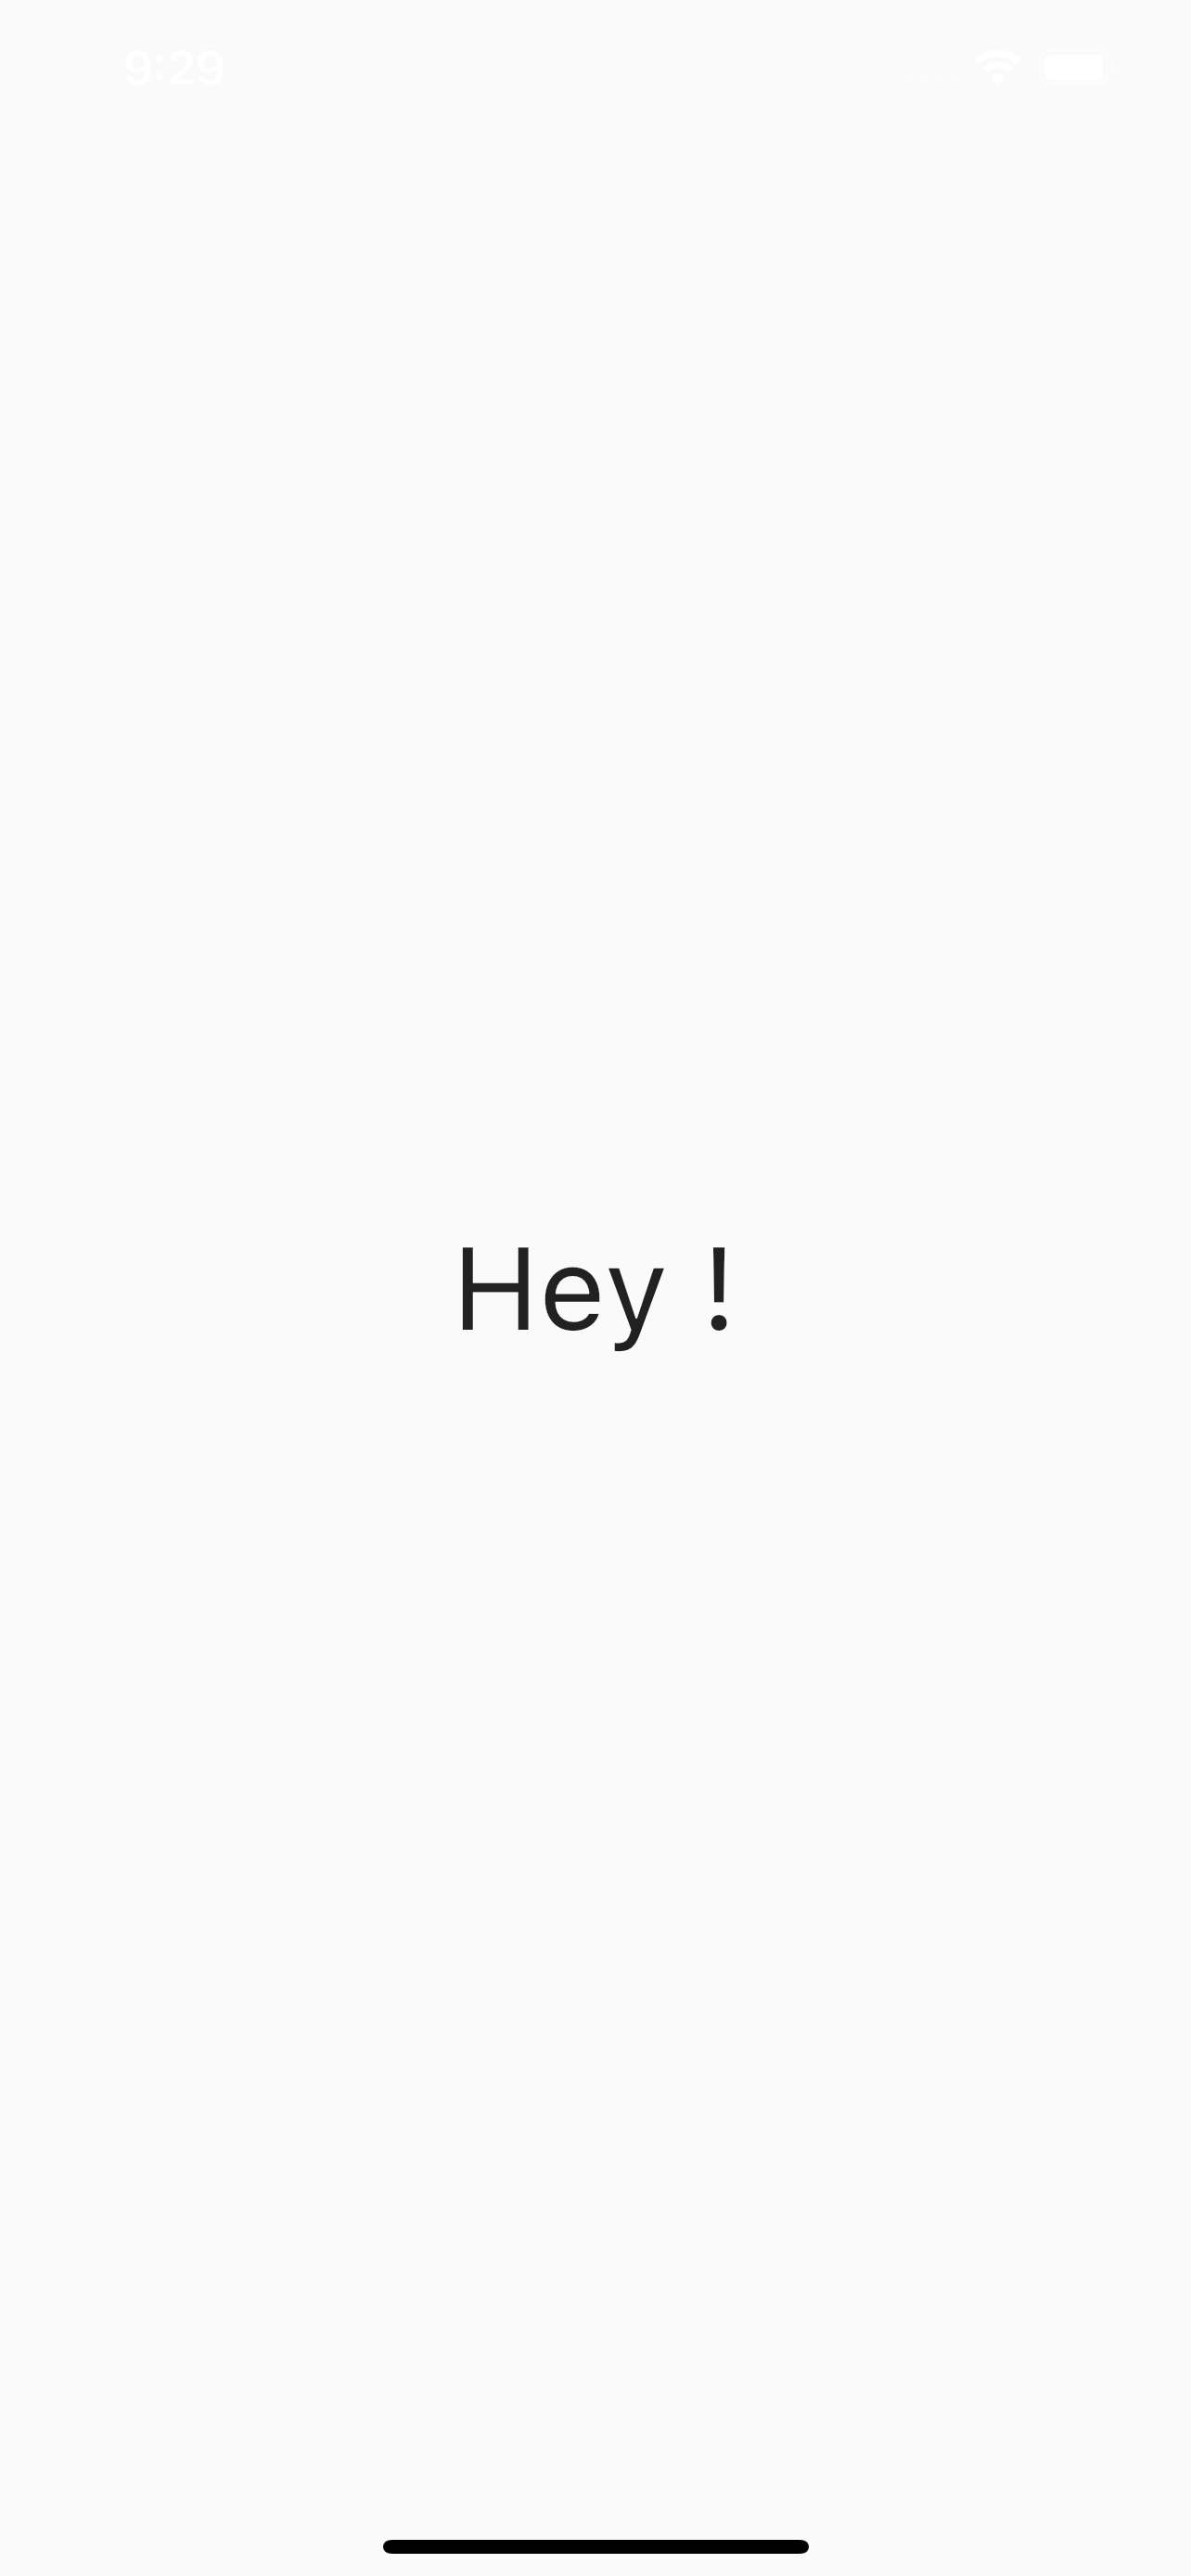
\includegraphics[width=0.60\textwidth]{../assets/img/Scaffold.jpg}
                \end{center}
            \end{figure}\end{column}
    \end{columns}
\end{frame}


\subsection{AppBar}
\begin{frame}[fragile,t]{\secname : \subsecname}
    \begin{columns}
        \begin{column}{0.5\textwidth}
            \begin{itemize}
                \item L'\href{https://api.flutter.dev/flutter/material/AppBar-class.html}{AppBar} est un widget;
                \item Se situer en haut de l’écran;
                \item Enfant de \emph{Scaffold}.
            \end{itemize}
            \begin{lstlisting}[language=C]
    return Scaffold(
        appBar: AppBar(
            title: Text(widget.title),
        ),
        body: Text("Hey"),
    );
    \end{lstlisting}
        \end{column}
        \begin{column}{0.5\textwidth}
            \begin{figure}
                \begin{center}
                    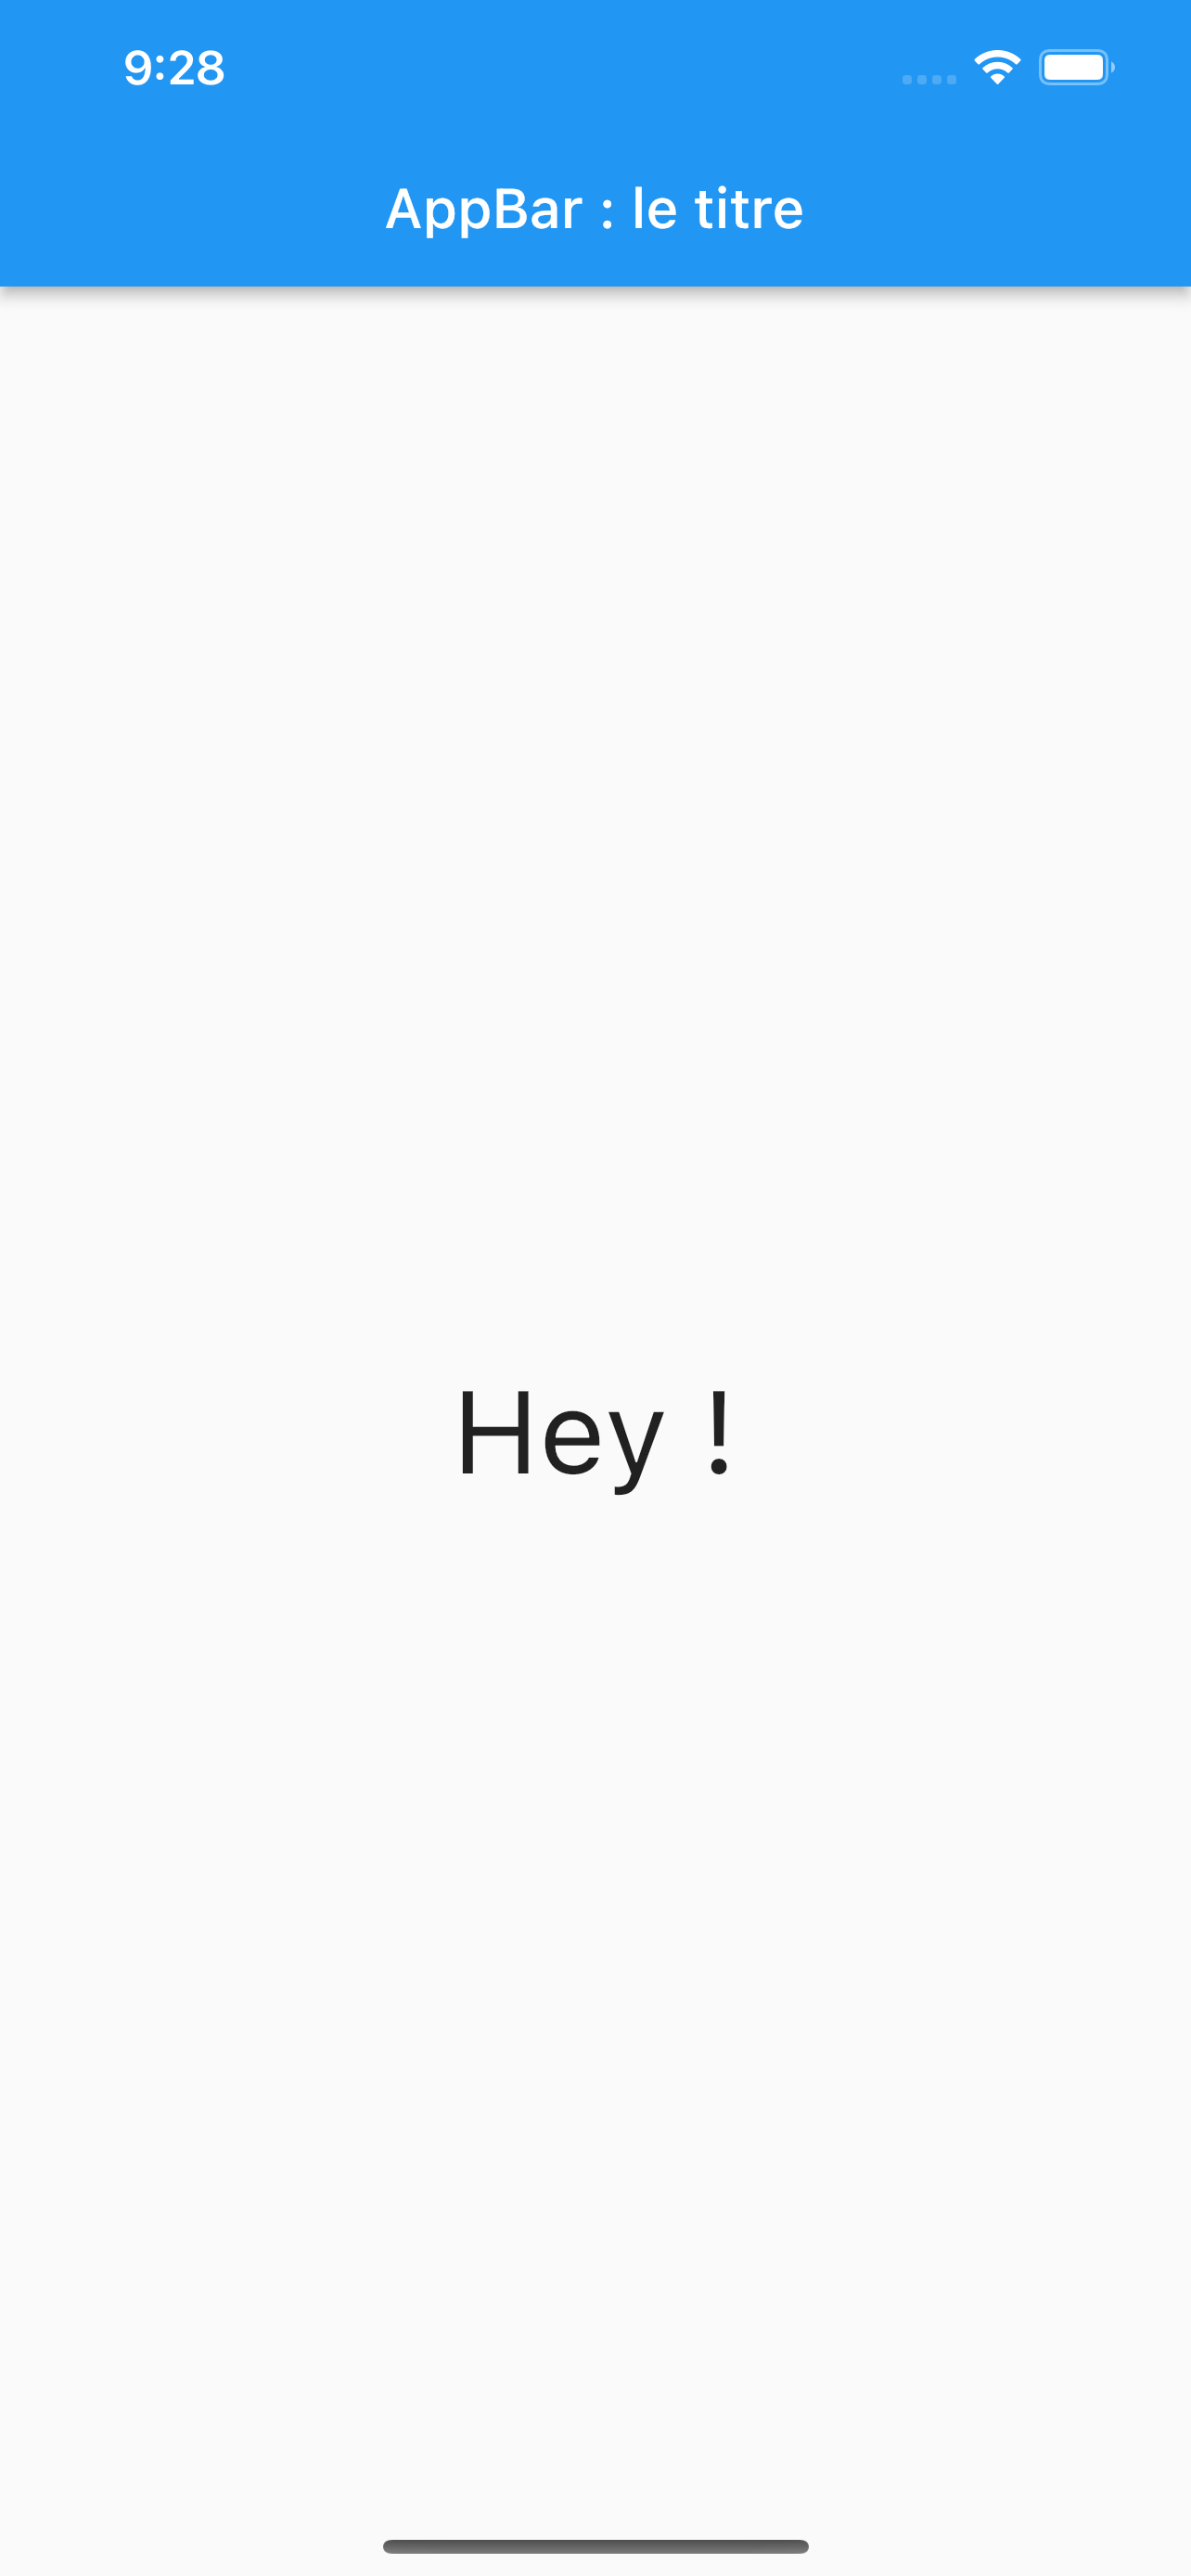
\includegraphics[width=0.60\textwidth]{../assets/img/AppBar.jpg}
                \end{center}
            \end{figure}\end{column}
    \end{columns}
\end{frame}

\subsection{floatingActionButton}
\begin{frame}[fragile,t]{\secname : \subsecname}
    \begin{columns}
        \begin{column}{0.6\textwidth}
            \begin{itemize}
                \item Le \href{https://api.flutter.dev/flutter/material/FloatingActionButton-class.html}{floatingActionButton} est un widget;
                \item Consiste en un bouton flottant;
                \item Qui peut être placé : centerDocked, bottomNavigationBar, centerFloat, endDocked,bottomNavigationBar, bottomNavigationBar, endTop,miniStartTop, startTop.
            \end{itemize}

            \begin{lstlisting}[language=C]
    floatingActionButton: FloatingActionButton(
        onPressed: () => {print("Bonjour")},
        child: const Icon(Icons.add),
        ),
    \end{lstlisting}
        \end{column}
        \begin{column}{0.4\textwidth}
            \begin{figure}
                \begin{center}
                    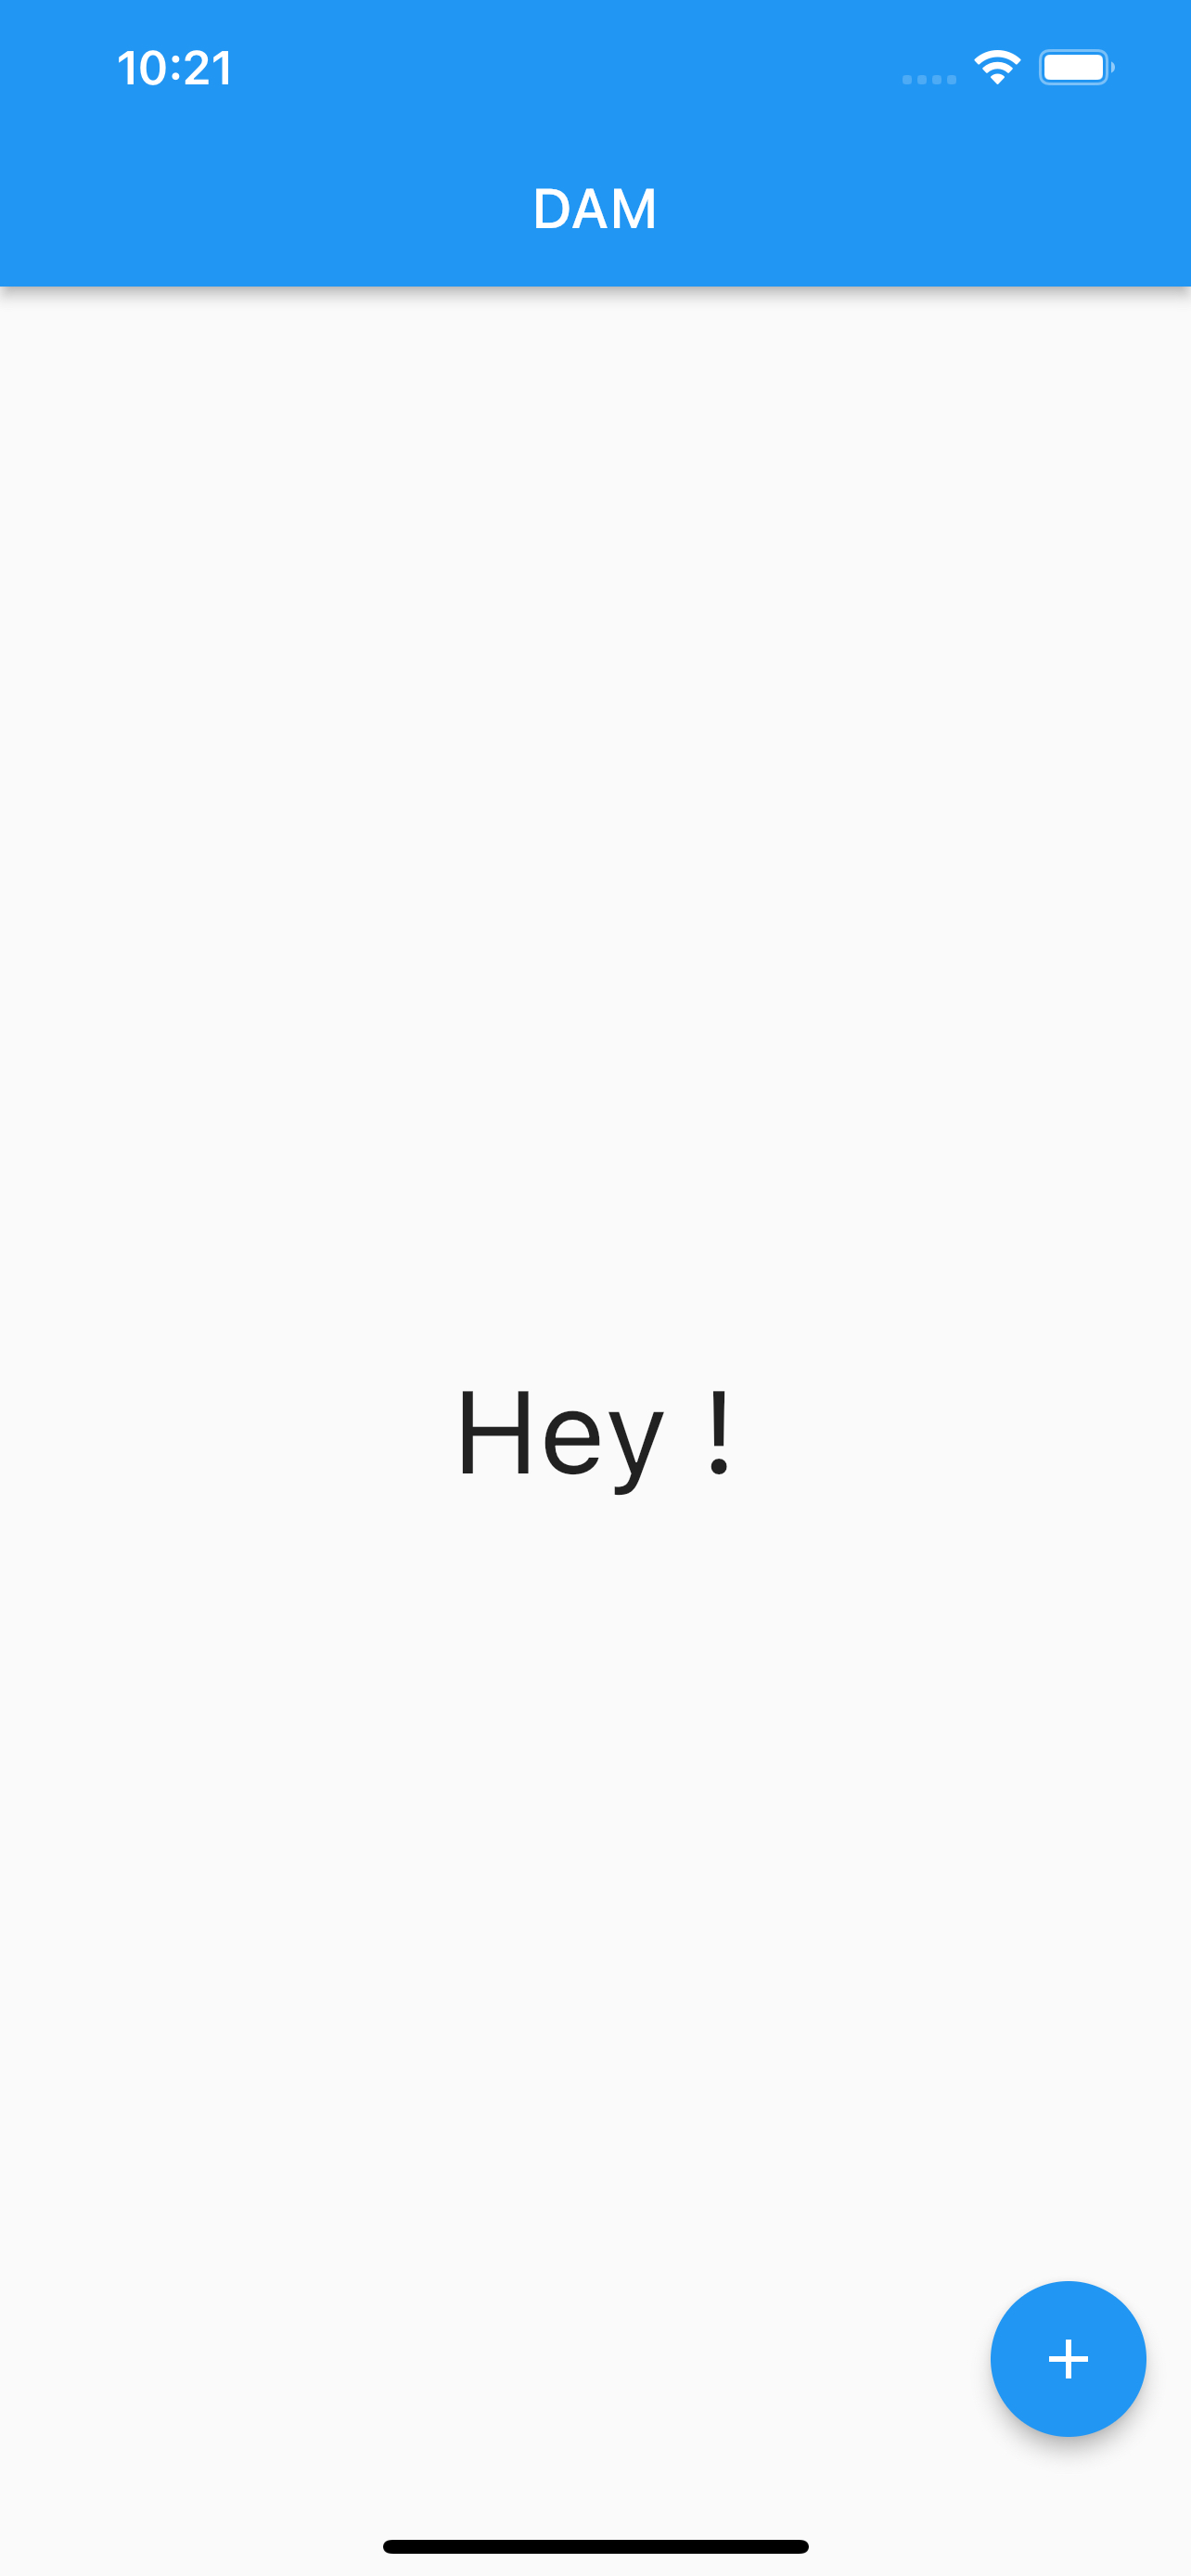
\includegraphics[width=0.60\textwidth]{../assets/img/floatingActionButton.jpg}
                \end{center}
            \end{figure}\end{column}
    \end{columns}
\end{frame}

\subsection{bottomNavigationBar}
\begin{frame}[fragile]{\secname : \subsecname}
    \begin{columns}
        \begin{column}{0.6\textwidth}
            \begin{itemize}
                \item La \href{https://api.flutter.dev/flutter/material/BottomNavigationBar-class.html}{bottomNavigationBar} est une barre de navigation;
                \item Située en bas de l’écran;
                \item Par défaut, sa taille est nulle;
                \item Il convient d’y inclure un Container par exemple;
            \end{itemize}
        \end{column}
        \begin{column}{0.4\textwidth}
            \begin{figure}
                \begin{center}
                    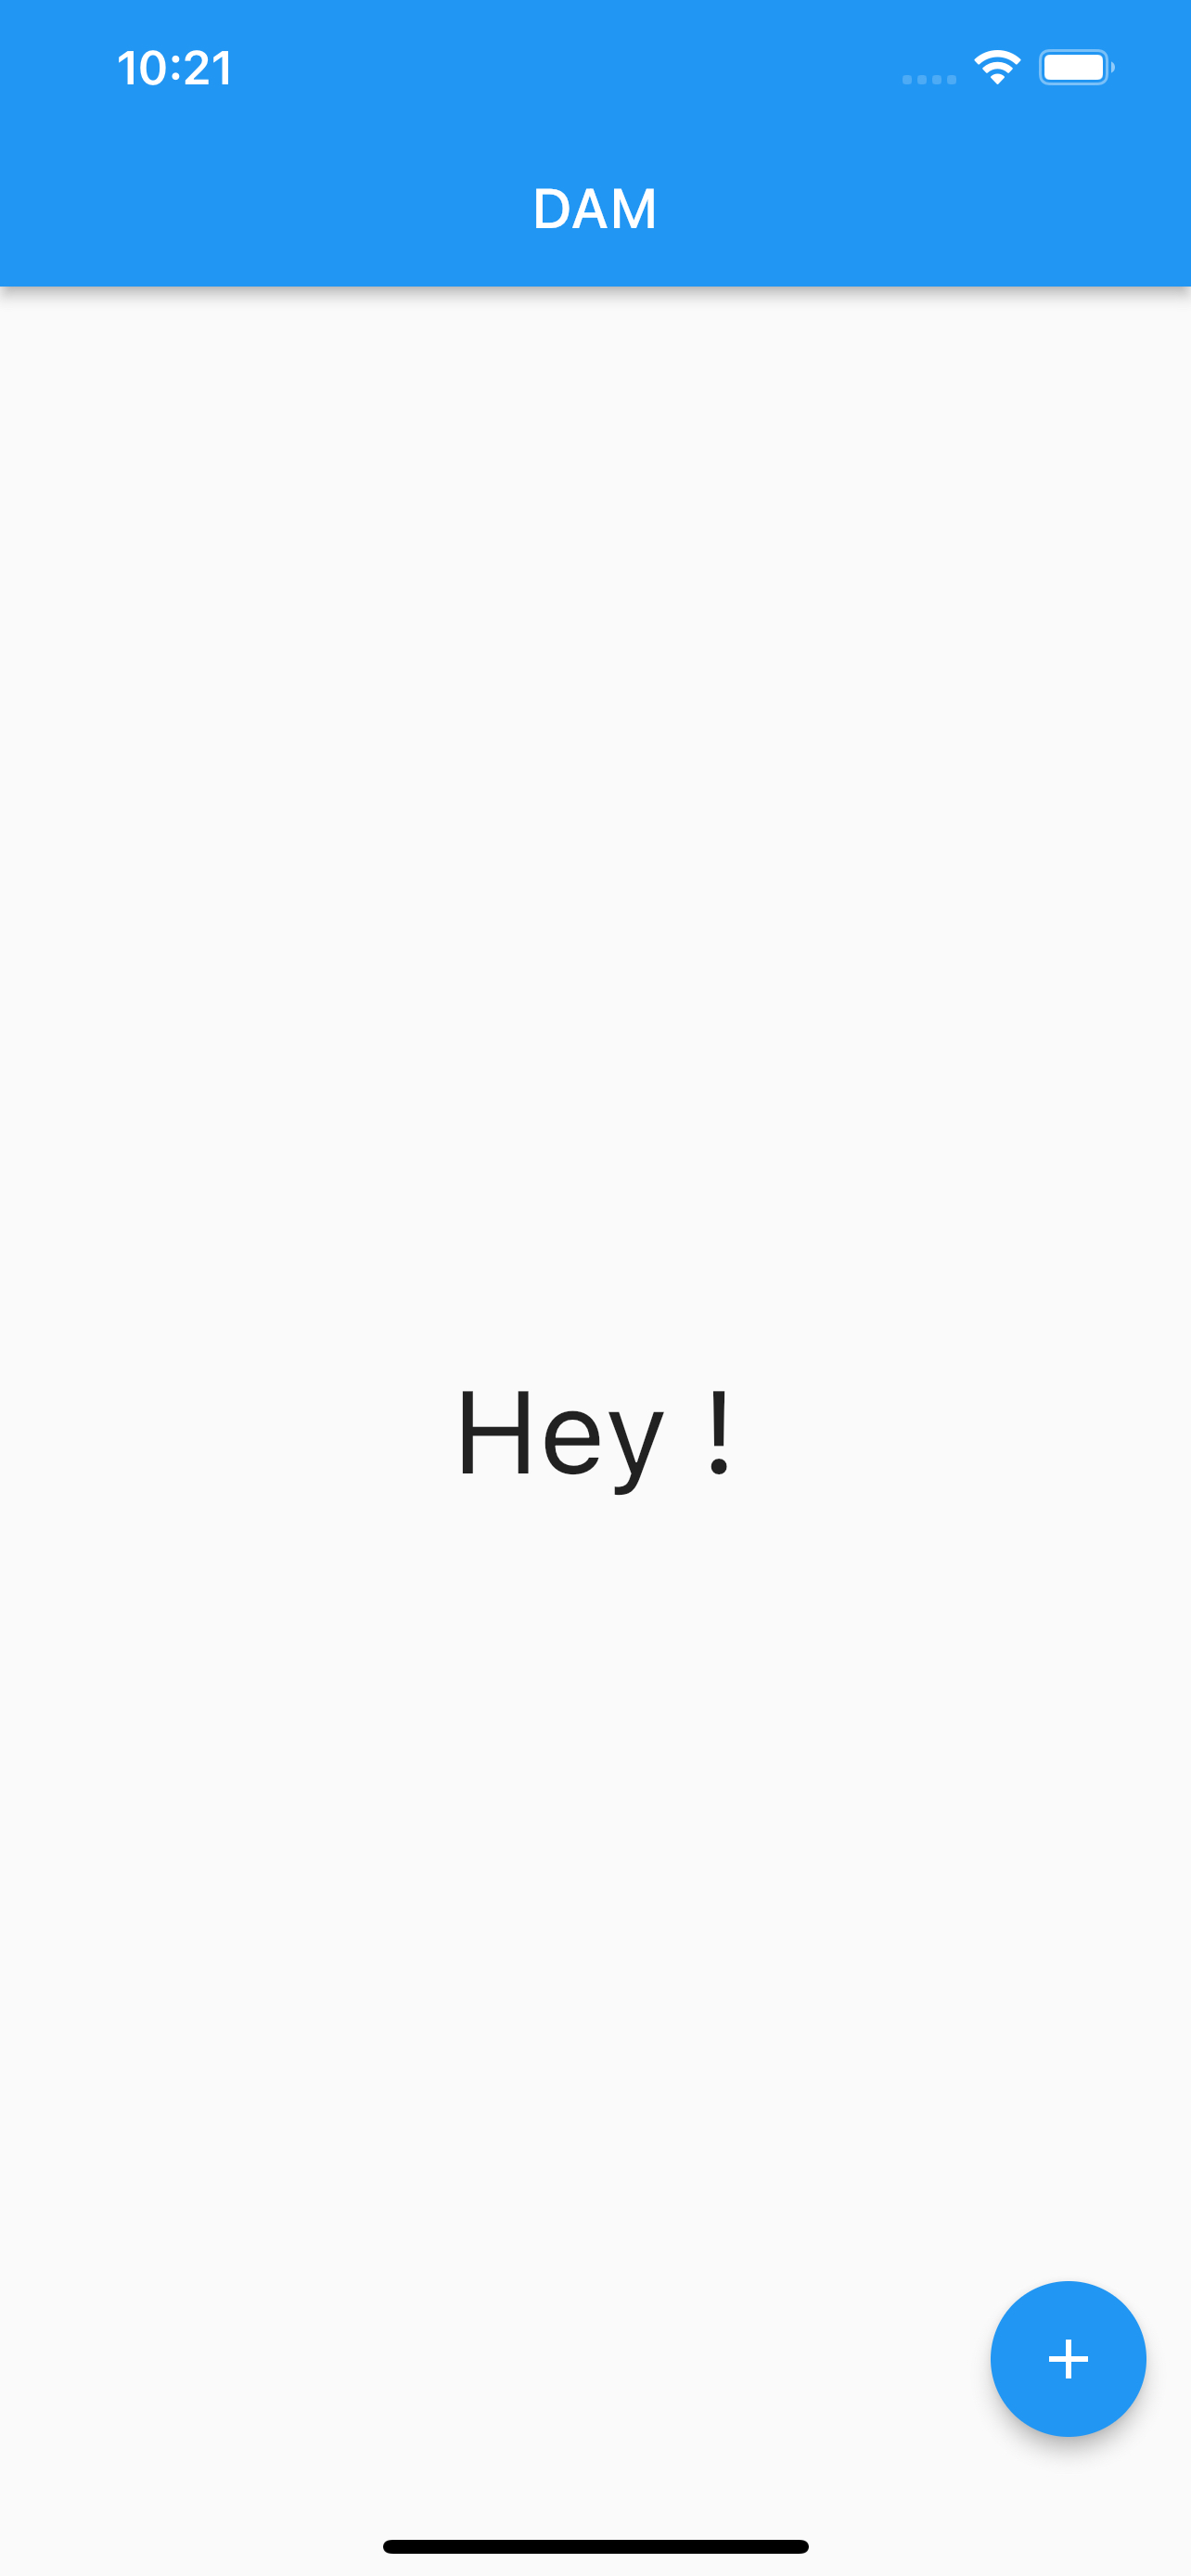
\includegraphics[width=0.60\textwidth]{../assets/img/floatingActionButton.jpg}
                \end{center}
            \end{figure}\end{column}
    \end{columns}
\end{frame}

\begin{frame}[fragile]{\secname : \subsecname}
    \begin{lstlisting}[language=C]
floatingActionButtonLocation: FloatingActionButtonLocation.centerDocked,
bottomNavigationBar: BottomAppBar(
    shape: CircularNotchedRectangle(),
    child: Container(
    height: 50,
    child: Row(
        mainAxisAlignment: MainAxisAlignment.spaceAround,
        children: [
        IconButton(
            onPressed: pressed,
            icon: Icon(Icons.add_location),
        ),
        IconButton(
            onPressed: pressed,
            icon: Icon(Icons.forward),
        ),],),),),
    \end{lstlisting}
\end{frame}


\section{Cupertino (Style iOS)}
\begin{frame}[fragile]{\secname}
    \begin{itemize}
        \item Style présent sur iOS;
        \item Nom donné en référence à la ville où se situe le siège d’Apple;
    \end{itemize}
    Nous ne couvrons pas ces widgets.
\end{frame}

\section{Détection de la plateforme}
\begin{frame}[fragile]{\secname}
    \begin{itemize}
        \item Pour se fondre dans le style de son système d’exploitation hôte, il convient alors de lui faire posséder les deux styles : Material Design et Cupertino;
        \item Créer deux Widgets, un pour Android et l’autre pour iOS;
        \item Il faut importer \lstinline[language=c]!Platform!.
    \end{itemize}
\end{frame}

\begin{frame}[fragile]{\secname}
    Ces propriétés retournent \lstinline[language=c]!true! si la plateforme est détectée au runtime.
    \begin{itemize}
        \item \lstinline[language=c]!Platform.isAndroid! pour détecter si le programme s’exécute sur;
        \item \lstinline[language=c]!Platform.isFuchsia! pour détecter si le programme s’exécute sur Fuchsia;
        \item \lstinline[language=c]!Platform.isIOS! pour détecter si le programme s’exécute sur iOS;
        \item \lstinline[language=c]!Platform.isLinux! pour détecter si le programme s’exécute sur Linux;
        \item \lstinline[language=c]!Platform.isMacOS! pour détecter si le programme s’exécute sur macOS.
    \end{itemize}
\end{frame}
\begin{frame}[fragile]{\secname}
    \begin{lstlisting}[language=C]
@override
Widget build(BuildContext context) {
return Platform.isIOS ? myCupertinoApp() : myCupertinoApp();
}
    \end{lstlisting}
    \lstinline[language=c]!myCupertinoApp! et \lstinline[language=c]!myCupertinoApp! étant des classes \lstinline[language=sql]!Widget! personelles.
\end{frame}
\section{Médias}
\begin{frame}[fragile]{\secname}
    \begin{itemize}
        \item Il est donc primordial de savoir intégrer des médias;
        \item Les icônes sont l’un des outils les plus employés de nos jours;
        \item Elles permettent d’obtenir une compréhension rapide simplement au travers d’un visuel;
        \item Des conventions se sont mises en place.
    \end{itemize}
\end{frame}

\subsection{Icônes}
\begin{frame}[fragile]{\secname : \subsecname}
    \begin{itemize}
        \item L’insertion de l’icône peut être réalisée au travers du widget \lstinline[language=sql]!Icon!;
        \item Ce dernier permet :
              \begin{itemize}
                  \item De définir la taille;
                  \item Sa couleur.
              \end{itemize}
        \item Flutter offre un vaste choix d’icônes;
        \item Soit en travaillant avec la classe Icons qui comporte une collection au style Material Design;
        \item soit avec la \lstinline[language=sql]!classeCupertinoIcons! qui propose un style iOS.

    \end{itemize}
    \begin{lstlisting}[language=C]
const Icon(
    Icons.notifications,
    size: 16,
    color: kMainTextColor,
),
        \end{lstlisting}
\end{frame}

\begin{frame}[fragile]{\secname : \subsecname}
    \begin{center}
        Il est possible de retrouver l’ensemble de ces icônes \linebreak
        \href{https://material.io/resources/icons/?style=baseline}{material.io/resources/icons}
    \end{center}
\end{frame}
\subsection{FontAwesome}
\begin{frame}[fragile]{\secname : \subsecname}
    \begin{itemize}
        \item \href{https://fontawesome.com}{FontAwesome} est un site Internet bien connu des développeurs web.
        \item Il offre une collection très importante d’icônes en tout genre.
    \end{itemize}
\end{frame}

\begin{frame}[fragile]{\secname : \subsecname}
    \begin{figure}
        \begin{center}
            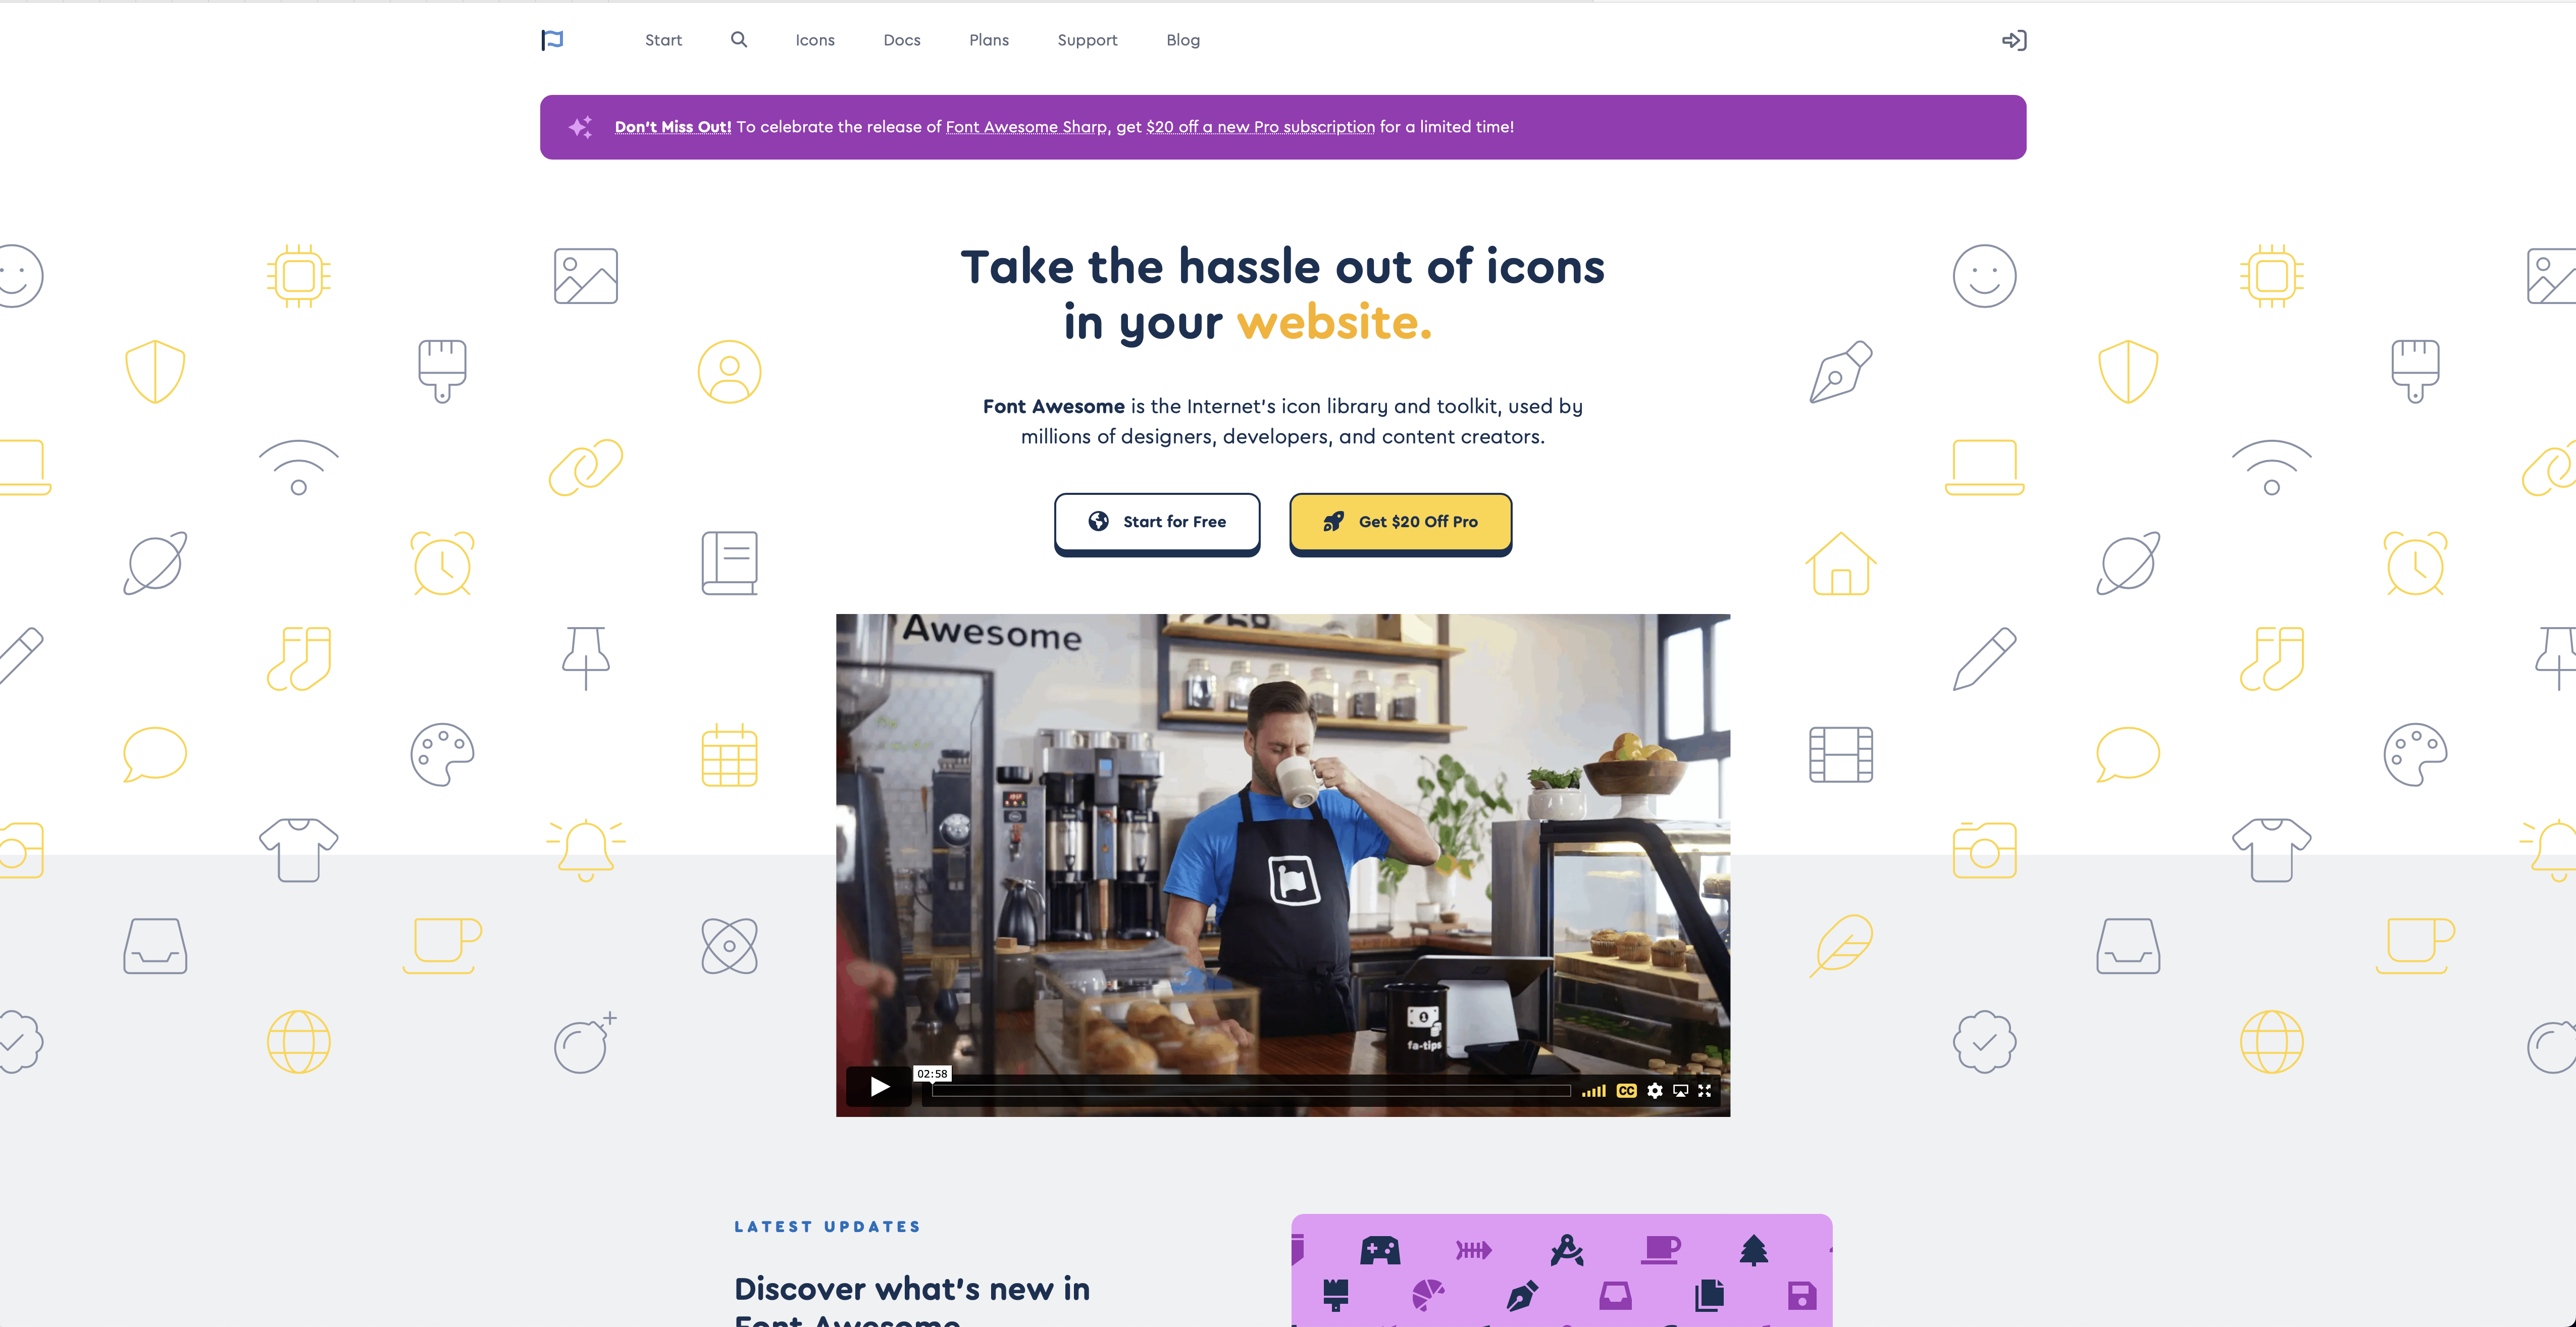
\includegraphics[width=\textwidth]{../assets/img/FontAwesome.jpg}
        \end{center}
    \end{figure}
\end{frame}

\begin{frame}[fragile]{\secname : \subsecname}
    \begin{figure}
        \begin{center}
            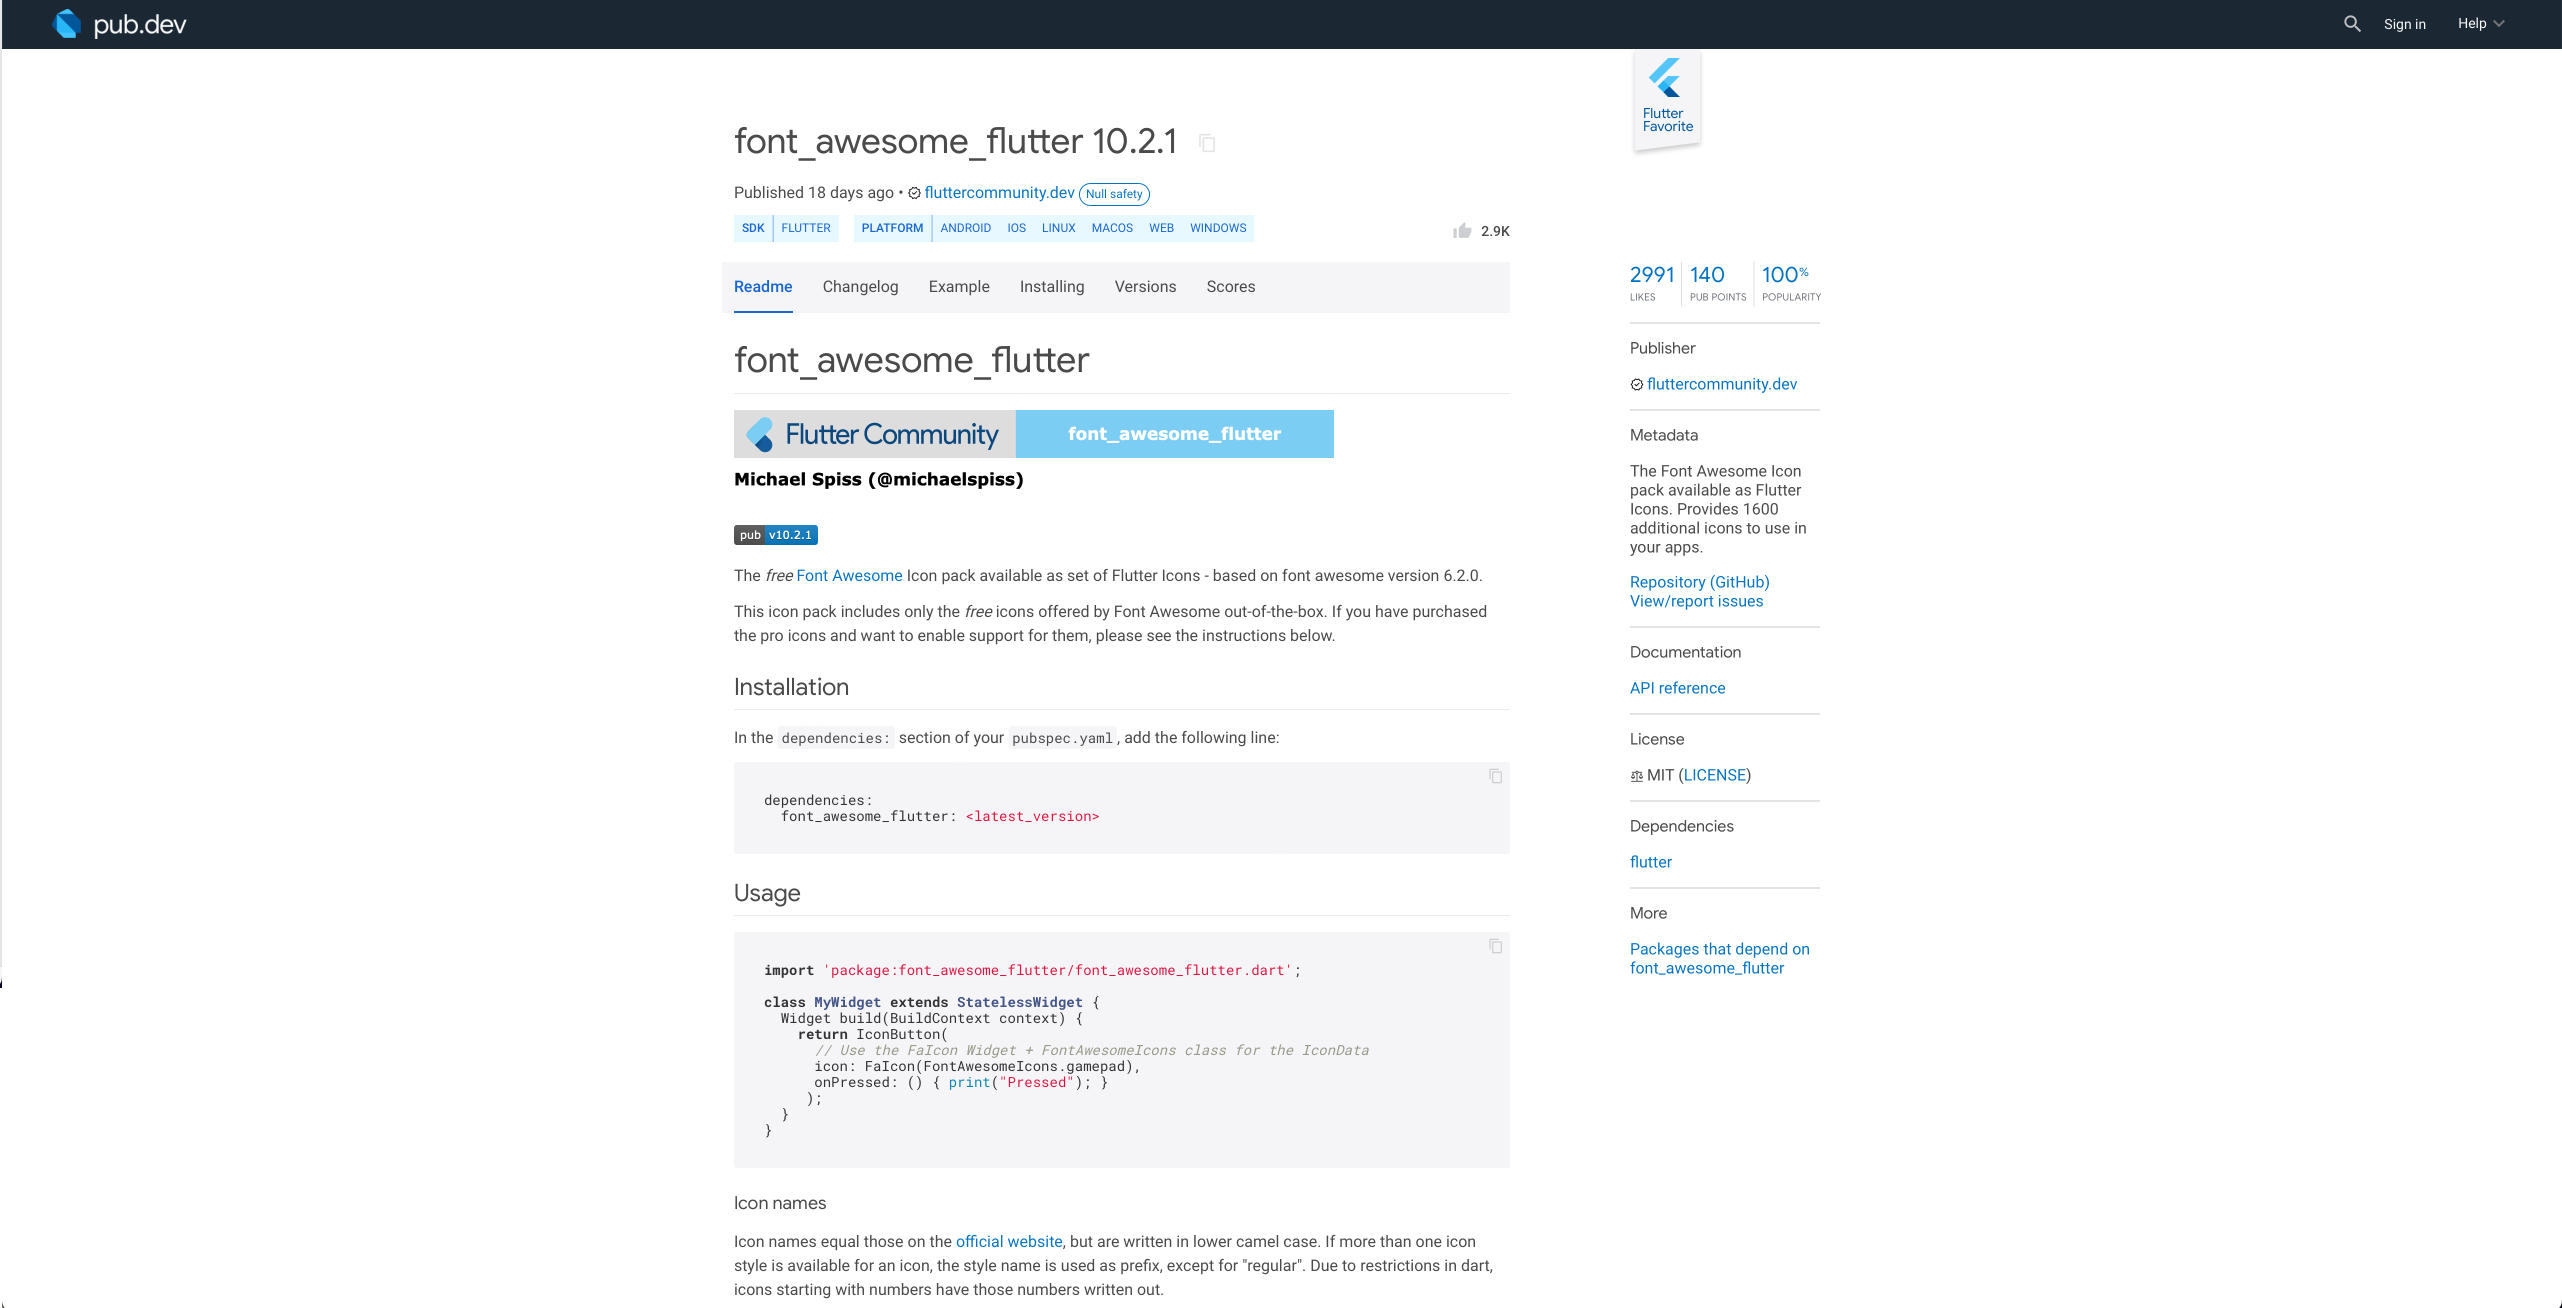
\includegraphics[width=\textwidth]{../assets/img/FontAwesome--pub-dev.jpg}
        \end{center}
    \end{figure}
\end{frame}

\section{Images}
\begin{frame}[fragile]{\secname}
    \begin{itemize}
        \item Pour rendre une application agréable en termes d’expérience utilisateur, il est courant d’insérer des images.
        \item Pour cela, plusieurs constructeurs nommés sont mis à disposition.
        \item Ils correspondent aux différents types de provenance d’une image, celles incluses au projet ou celles venant directement du web.
    \end{itemize}
\end{frame}
\subsection{Web}
\begin{frame}[fragile]{\secname : \subsecname}
    \begin{lstlisting}[language=C]
ClipRRect(
borderRadius: kBorderRadiusItem,
    child: Image.network(
        'https://image.tmdb.org/t/p/w154/$path',
        height: 230,
        width: 154,
    ),
),
\end{lstlisting}
\end{frame}
\subsection{Statique}
\begin{frame}[fragile]{\secname : \subsecname}
    \begin{lstlisting}[language=C]
Image.asset(
    'assets/img/actor_placeholder.jpg',
    height: 190,
    width: 154,
    fit: BoxFit.fitWidth,
);
\end{lstlisting}
    \begin{alertblock}{Attention}
        Il faut impérativement charger l'image dans l'application depuis le fichier \emph{pubspec.yaml}.
    \end{alertblock}
\end{frame}

\section{Polices de caractères}
\begin{frame}[fragile]{\secname}
    Pour charger une police de caractères, il faut :
    \begin{itemize}
        \item Télécharger les fichiers dans un dossier du projet;
        \item Déclarer la police de caractères dans le fichier \emph{pubspec.yaml};
        \item Utiliser la police de caractères dans un widget spécifique.
    \end{itemize}
    \begin{lstlisting}[language=C]
awesome_app/
    fonts/
        Raleway-Regular.ttf
        Raleway-Italic.ttf
        RobotoMono-Regular.ttf
        RobotoMono-Bold.ttf
\end{lstlisting}
\end{frame}

\begin{frame}[fragile]{\secname}
    Définir une police par défaut
    \begin{lstlisting}[language=C]
return MaterialApp(
    title: 'Custom Fonts',
    // Ici
    theme: ThemeData(fontFamily: 'Raleway'),
    home: const MyHomePage(),
    );
\end{lstlisting}
\end{frame}

\end{document}